\documentclass[12pt]{article}
\usepackage[utf8]{inputenc}
\usepackage[T1]{fontenc}
\usepackage[ngerman]{babel}
\usepackage{lmodern}
\usepackage{svg}
\usepackage{hyperref}

\graphicspath{ {./images} }

\title{Eigenes Betriebssystem : Dokumentation}
\author{Maximilian Trautwein}

\begin{document}
	
	\maketitle
	
	\begin{figure}[h]
		\centering
		
\includegraphics[width=\textwidth]{FBS-Logo_2021-1}
	\end{figure}
	
	\newpage
	\tableofcontents
	
	\newpage
	
	\section{UEFI / BIOS}
	Die erste Grundfrage, die ich mir gestellt habe, ist, ob ich einen BIOS\cite{bios} oder UEFI Bootloader\cite{uefi} programmiere. Ich habe mich für einen UEFI-Bootloader\cite{uefi} entschieden, da das originale BIOS\cite{bios} nicht sehr viele Möglichkeiten zur Interaktion mit der Hardware bietet und ich mit dem UEFI\cite{uefi} auf der sicheren und fortschrittlicheren Seite bin. 
	\subsection{BIOS}
 	Das BIOS\cite{bios} (Basic Input Output System) ist ein von IBM in 1981 zuerst implementiertes und in 1975 von Gary Kildall erdachtes System, welches Entwicklern helfen soll, einfacher und unabhängiger auf die Hardware zuzugreifen und somit die Betriebssystementwicklung normierter und weniger komplex zu gestalten. Das BIOS\cite{bios} stellt Funktionen und Felder zur Verfügung, mit denen man z.B. Text ausgeben oder einfachen Zugriff auf Speicher zum Starten eines Betriebssystems haben kann. 
 	\subsection{UEFI} 
 	Das UEFI\cite{uefi} (Unified Extensible Firmware Interface) ist eine Firmwaredefinition für x86-64 , ARM und Itanium Architekturen. Diese definiert eine Schnittstelle zwischen BIOS\cite{bios} und dem Betriebssystem. Ursprünglich hat Intel diese Firmware für ihre Itanium-Platform entwickelt und hat 2005 eine Gruppe (Unified EFI Forum) gebildet, welche aus allen großen Hardwarefirmen besteht (AMD, Intel, Microsoft und Apple).
	
	\newpage
	
	\section{Bootloader}
	Der Bootloader\cite{bootloader} ist ein kleines Programm, welches den Kernel\cite{kernel} aus einer Partition einliest und die Eingangsfunktion dieses Kernels\cite{kernel} aufruft und dem Kernel\cite{kernel} die Kontrolle über die Hardware erteilt. Außerdem wechselt er zum kernelspezifischen Betriebsmodus. Das BIOS/UEFI\cite{uefi} bestimmt, wie der Bootloader\cite{bootloader} programmiert wird und wie dieser die Kontrolle übergibt.
	Die zweite Grundfrage, die ich mir gestellt habe, ist, ob ich einen eigenen Bootloader\cite{bootloader} programmieren sollte oder lieber auf schon vorhandene Bootloader\cite{bootloader} zurückgreife. Ich habe mich für einen eigenen Bootloader\cite{bootloader} entschieden, da ich somit mehr lerne und auch mehr Kontrolle darüber habe, wie und was etwas ausgeführt wird. Für die Entwicklung von UEFI\cite{uefi}-Applikationen gibt es eine Entwicklungsumgebung aus dem GNU-Projekt, das "gnu-efi" heisst. Diese Umgebung bietet einen effizienten Zugriff auf Funktionen und Informationen aus dem UEFI\cite{uefi}.
	
	\section{Entwicklungsumgebung}
	Da ich platformunabhängige Software programmiere, brauche ich einen Cross-Compiler. Als C/C++ Compiler nutze ich GCC/G++, da diese auch ohne spezifische Platform ausführbare Dateien kompilieren kann. Als Code-Editor habe ich VS-Code verwendet, da ich auf Windows mit WSL mein Betriebssystem kompiliere. VS-Code unterstützt das Verbinden von dem Editor und WSL. Das ermöglicht einem die richtigen Vervollständingungen und Einfärbungen des Codes, damit die Programmierung angenehmer und effizienter verläuft. Als Testumgebung habe ich QEMU, ein Systememulator und virtuelle Maschine, welche mit der OVMF (Open Virtual Machine Firmware) ausgeführt wird, damit auch UEFI\cite{uefi}-Systeme emuliert werden können. Der Cross-Compiler erschafft eine Image-Datei, welche QEMU dann ausführt. 
	
	\newpage
	
	\section{Allgemeine Konzepte und Begriffe}
	\subsection{Kernel}
	Der Kernel\cite{kernel} ist die zentrale Einheit eines Betriebssystems und verwaltet Speicher/Arbeitsspeicher, Geräte und bietet eine Schnittstelle für Programme von Nutzern. Der Kernel\cite{kernel} erhält diese Informationen vom BIOS/UEFI\cite{uefi}.
	\subsection{GOP}
	Das GOP\cite{gop} (General Output Protocol) ist ein UEFI\cite{uefi} Protokoll für den einfachen Zugriff auf den Bildschirm, um Text auszugeben. Das Buffer kann man an den Kernel\cite{kernel} weitergeben, damit dieser einfach die Pixel auf dem Bildschirm setzen kann. 
	\subsection{Paging}
	Paging\cite{paging} ist ein Arbeitsspeicherverwaltungssystem, das virtuelle Speicheradressen zu physischen Adressen setzt. Dadurch kann man Arbeitsspeicherbereiche für jede Applikation auf dem Betriebssystem erstellen und somit diese isolieren. Somit kann eine Applikation nicht den reservierten Arbeitsspeicher einer anderen korrumpieren. Das umadressieren erledigt die MMU(Memory Management Unit), welche sich auf der CPU befindet.
	\begin{figure}[h]
		\centering
		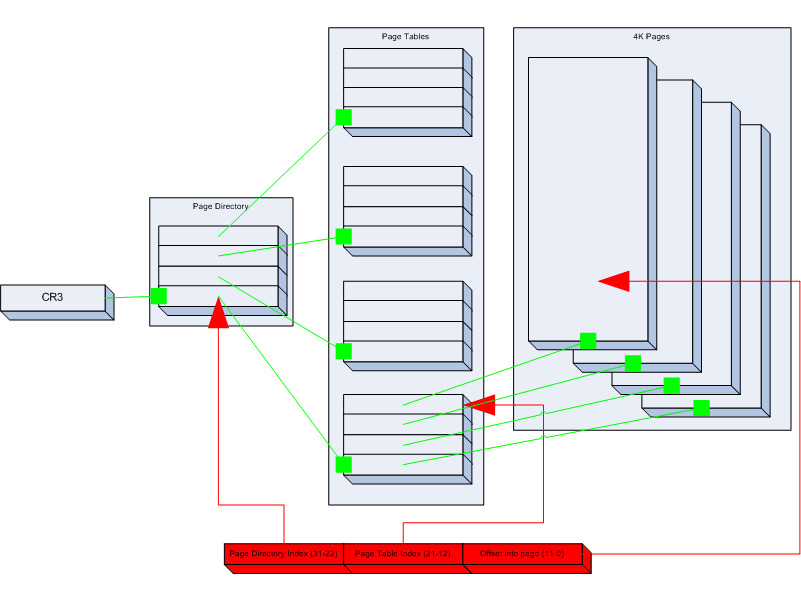
\includegraphics[width=9cm]{paging}
	\end{figure}
	\newpage
	\subsection{Interrupts}
	Interrupts\cite{interrupts} sind Anfragen von Geräte an die CPU, dass sie ihre derzeitige Aufgabe stoppen und mit etwas anderem, z.B. das Ausführen einer anderen Funktion, beginnen soll. Nach dem Sprung zur anderen Funktion kann die CPU wieder bei der letzten ausgeführten Anweisung fortfahren.
	\subsection{PCI}
	PCI\cite{pci} (Peripheral Component Interconnect) ist eine Bus-Art, welche zur Datenübertragung und zur Steuerung von Geräten genutzt wird. Durch einen PCI\cite{pci}-Bus kann man auch Geräte-IDs abrufen und mit einer Datenbank vergleichen, um z.B. den richtigen Treiber anzuwenden. Man kann auch Geräte ausschalten.
	\subsection{GDT}
	Der GDT\cite{gdt} (Global Descriptor Table) ist eine Datenstruktur spezifisch für IA-32 und x86-64, die die MMU darüber informiert, welche Arbeitsspeichersegmente von dem UEFI\cite{uefi} erkannt wurden. Es setzt den Schreibschutz für diese Segmente, damit verschiedene Applikationen ihren eigenen Sicherheitsbereich haben. 
	\subsection{IDT}
	Der IDT\cite{idt} (Interrupt Descriptor Table) ist auch eine Datenstruktur, die auch nur auf IA-32 und x86-64 existiert. Sie sagt aus, welche Funktionen von welchen Interrupts\cite{interrupts} aufgerufen werden. Diese Funktionen müssen natürlich auch existieren. GCC enthält ein Funktionenattribut namens "interrupt", womit man diese Funktionen auch in C definieren kann und somit Assembly umgeht.
	
	\newpage
	
	\begin{thebibliography}{10}
		
		\bibitem{kernel} \url{https://wiki.osdev.org/Kernel}
		\bibitem{gop} \url{https://wiki.osdev.org/GOP}
		\bibitem{bootloader} \url{https://wiki.osdev.org/Bootloader}
		\bibitem{paging} \url{https://wiki.osdev.org/Paging}
		\bibitem{interrupts} \url{https://wiki.osdev.org/Interrupts}
		\bibitem{pci} \url{https://wiki.osdev.org/Pci}
		\bibitem{gdt} \url{https://wiki.osdev.org/GDT}
		\bibitem{idt} \url{https://wiki.osdev.org/IDT}
		\bibitem{uefi} \url{https://wiki.osdev.org/UEFI}
		\bibitem{bios} \url{https://wiki.osdev.org/BIOS}
		\bibitem{poncho} \url{https://www.youtube.com/@poncho2364}
		\bibitem{osdev} \url{https://wiki.osdev.org/Main_Page}
		
	\end{thebibliography}
	
\end{document}